\documentclass{article}
\usepackage{v-test-paper}

\renewcommand{\frac}[2]{\dfrac{#1}{#2}}

\newenvironment{solution}{\par\noindent\color{red!85!black}$\Rightarrow$\vspace{0em}}{}

\title{\textsc{JEE Advanced 2023 Paper-II\\Physics}}
\date{}


\begin{document}
\maketitle

\begin{enumerate}
    \item An electric dipole is formed by two charges \(+q\) and \(-q\) located in xy-plane at \((0,2)\) mm and \((0,-2)\) mm, respectively, as shown in the figure. The electric potential at point \(P\) \((100,100)\) mm due to the dipole is \(V_0\). The charges \(+q\) and \(-q\) are then moved to the points \((-1,2)\) mm and \((1,-2)\) mm, respectively. What is the value of electric potential at \(P\) due to the new dipole?
        \begin{tasks}(2)
        	\task \(V_0/4\)
        	\task \(V_0/2\)
        	\task \(V_0/\sqrt{2}\)
        	\task \(3V_0/4\)
        \end{tasks}
    \item Young's modulus of elasticity \(Y\) is expressed in terms of three derived quantities, namely, the gravitational constant \(G\), Planck's constant \(h\) and the speed of light \(c\), as \(Y = c^\alpha h^\beta G^\gamma\). Which of the following is the correct option?
        \begin{tasks}(2)
        	\task \(\alpha = 7, \beta = -1, \gamma = -2\)
        	\task \(\alpha = -7, \beta = -1, \gamma = -2\)
        	\task \(\alpha = 7, \beta = -1, \gamma = 2\)
        	\task \(\alpha = -7, \beta = 1, \gamma = -2\)
        \end{tasks}
    \item A particle of mass \(m\) is moving in the \(xy\)-plane such that its velocity at a point \((x,y)\) is given as \(\vec{v} = \alpha(y\hat{x} + 2x\hat{y})\), where \(\alpha\) is a non-zero constant. What is the force \( \vec{F} \) acting on the particle?
        \begin{tasks}(2)
        	\task \(\vec{F} = 2ma\alpha(x\hat{x} + y\hat{y})\)
        	\task \(\vec{F} = m\alpha^2(y\hat{x} + 2x\hat{y})\)
        	\task \(\vec{F} = 2ma\alpha(y\hat{x} + x\hat{y})\)
        	\task \(\vec{F} = ma\alpha(x\hat{x} + 2y\hat{y})\)
        \end{tasks}
    \begin{center}
        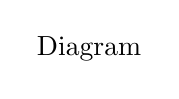
\begin{tikzpicture}
            \node {Diagram};
        \end{tikzpicture}
    \end{center}
    

    \item An ideal gas is in thermodynamic equilibrium. The number of degrees of freedom of a molecule of the gas is \( x \). The internal energy of one mole of the gas is \( U_x \), and the speed of sound in the gas is \( v_x \). At a fixed temperature and pressure, which of the following is the correct option?
        \begin{tasks}(2)
            \task \( v_3 < v_6 \) and \( U_3 > U_6 \)
            \task \( v_5 > v_3 \) and \( U_3 > U_5 \)
            \task \( v_5 > v_7 \) and \( U_5 < U_7 \)
            \task \( v_6 < v_7 \) and \( U_6 < U_7 \)
        \end{tasks}

    \item A monochromatic light wave is incident normally on a glass slab of thickness \(d\), as shown in the figure. The refractive index of the slab increases linearly from \(n_1\) to \(n_2\) over the height \(h\). Which of the following statement(s) is(are) true about the light wave emerging out of the slab?
        \begin{tasks}(1)
            \task It will deflect up by an angle \(\tan^{-1}\left[\frac{(n_2-n_1)d}{2h}\right]\).
            \task It will deflect up by an angle \(\tan^{-1}\left[\frac{(n_2-n_1)d}{h}\right]\).
            \task It will not deflect.
            \task The deflection angle depends only on \(n_2 - n_1\) and not on the individual values of \(n_1\) and \(n_2\).
        \end{tasks}
    \item An annular disk of mass \(M\), inner radius \(a\), and outer radius \(b\) is placed on a horizontal surface with a coefficient of friction \(\mu\), as shown in the figure. At some time, an impulse \(J_0\) is applied at a height \(h\) above the center of the disk. If \(h = h_m\), then the disk rolls without slipping along the x-axis. Which of the following statement(s) is(are) correct?
        \begin{tasks}(1)
            \task For \(\mu \neq 0\) and \(a \rightarrow 0\), \(h_m = \frac{b}{2}\).
            \task For \(\mu \neq 0\) and \(a \rightarrow b\), \(h_m = b\).
            \task For \(h = h_m\), the initial angular velocity does not depend on the inner radius \(a\).
            \task For \(\mu = 0\) and \(h = 0\), the wheel always slides without rolling.
        \end{tasks}

    \item The electric field associated with an electromagnetic wave propagating in a dielectric medium is given by $\vec{E} = 30(2 + \hat{j})\sin\left[2\pi(5 \times 10^{14}t - \frac{10^{7}}{3} z)\right] \mathrm{Vm}^{-1}$. Which of the following option(s) is(are) correct? (Given: The speed of light in vacuum, $c = 3 \times 10^{8} \mathrm{ms}^{-1}$)
        \begin{tasks}(2)
            \task $B_{x} = -2 \times 10^{-7}\sin\left[2\pi(5 \times 10^{14}t - \frac{10^{7}}{3} z)\right] \mathrm{Wbm}^{-2}$
            \task $B_{y} = 2 \times 10^{-7}\sin\left[2\pi(5 \times 10^{14}t - \frac{10^{7}}{3} z)\right] \mathrm{Wbm}^{-2}$
            \task The wave is polarized in the xy-plane with polarization angle $30^{\circ}$ with respect to the x-axis.
            \task The refractive index of the medium is 2.
        \end{tasks}

    \item A thin circular coin of mass 5 gm and radius 4/3 cm is initially in a horizontal xy-plane. The coin is tossed vertically up (+z direction) by applying an impulse of $\frac{\sqrt{3}}{2} \times 10^{-2}$ N-s at a distance 2/3 cm from its center. The coin spins about its diameter and moves along the +z direction. By the time the coin reaches back to its initial position, it completes n rotations. The value of n is \underline{\hspace{2em}}.
    
    \begin{center}
        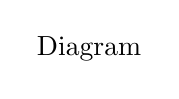
\begin{tikzpicture}
            \node {Diagram};
        \end{tikzpicture}
    \end{center}
    
    \item A rectangular conducting loop of length 4 cm and width 2 cm is in the xy-plane, as shown in the figure. It is being moved away from a thin and long conducting wire along the direction $\frac{\sqrt{3}}{2} \hat{i} + \frac{1}{2} \hat{j}$ with a constant speed v. The wire is carrying a steady current I = 10 A in the positive x-direction. A current of 10 $\mu$A flows through the loop when it is at a distance d = 4 cm from the wire. If the resistance of the loop is 0.1 $\Omega$, then the value of v is \underline{\hspace{2em}} m s$^{-1}$.
    
    \begin{center}
        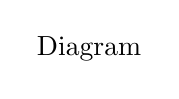
\begin{tikzpicture}
            \node {Diagram};
        \end{tikzpicture}
    \end{center}

    \item A string of length 1 m and mass \( 2 \times 10^{-5} \) kg is under tension \( T \). When the string vibrates, two successive harmonics are found to occur at frequencies 750 Hz and 1000 Hz. The value of tension \( T \) is \underline{\hspace{2cm}} Newton.
    \item An incompressible liquid is kept in a container having a weightless piston with a hole. A capillary tube of inner radius 0.1 mm is dipped vertically into the liquid through the airtight piston hole, as shown in the figure. The air in the container is isothermally compressed from its original volume \( V_0 \) to \( \frac{100}{101}V_0 \) with the movable piston. Considering air as an ideal gas, the height \( h \) of the liquid column in the capillary above the liquid level in cm is \underline{\hspace{2cm}}.

    \begin{center}
        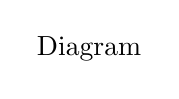
\begin{tikzpicture}
            \node {Diagram};
        \end{tikzpicture}
    \end{center}

    [Given: Surface tension of the liquid is 0.075 N m\(^{-1}\), atmospheric pressure is \( 10^5 \) N m\(^{-2}\), acceleration due to gravity (\( g \)) is 10 m s\(^{-2}\), density of the liquid is \( 10^3 \) kg m\(^{-3}\) and contact angle of capillary surface with the liquid is zero]
    \item In a radioactive decay process, the activity is defined as \( A = -\frac{dN}{dt} \) where \( N(t) \) is the number of radioactive nuclei at time \( t \). Two radioactive sources, \( S_1 \) and \( S_2 \), have same activity at time \( t = 0 \). At a later time, the activities of \( S_1 \) and \( S_2 \) are \( A_1 \) and \( A_2 \), respectively. When \( S_1 \) and \( S_2 \) have just completed their 3rd and 7th half-lives, respectively, the ratio \( \frac{A_1}{A_2} \) is \underline{\hspace{2cm}}.

    \item One mole of an ideal gas undergoes two different cyclic processes I and II, as shown in the P-V diagrams below. In cycle I, processes \(a\), \(b\), \(c\) and \(d\) are isobaric, isothermal, isobaric and isochoric, respectively. In cycle II, processes \(a'\), \(b'\), \(c'\) and \(d'\) are isothermal, isochoric, isobaric and isochoric, respectively. The total work done during cycle I is \(W_{\mathrm{I}}\) and that during cycle II is \(W_{\mathrm{II}}\). The ratio \(W_{\mathrm{I}}/W_{\mathrm{II}}\) is \_\_\_.
    
    \begin{center}
        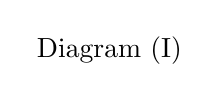
\begin{tikzpicture}
            \node {Diagram (I)};
        \end{tikzpicture}
    \end{center}
    
    \begin{center}
        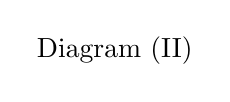
\begin{tikzpicture}
            \node {Diagram (II)};
        \end{tikzpicture}
    \end{center}
    
\end{enumerate}

\begin{center}
\texttt{Answer Key}
\begin{multicols}{5}
\begin{enumerate}
\item (b)
\item (b)
\item (a)
\item (b)
\item (d)
\item (b)
\item (c)
\item (a), (b)
\item (c)
\item (a), (b), (c), (d)
\end{enumerate}
\end{multicols}
\end{center}


\end{document}